\documentclass[12pt,a4paper]{article}

% ─── 1. PACKAGES ──────────────────────────────────────────────────────────────
\usepackage[utf8]{inputenc}
\usepackage[T1]{fontenc}
\usepackage{amsmath, amssymb}
\usepackage{geometry}
\usepackage{graphicx}
\usepackage{xcolor}
\usepackage{listings}
\usepackage{hyperref}
\usepackage{booktabs}
\usepackage{enumitem}
\usepackage{tcolorbox}
\usepackage{mdframed}
\usepackage{fancyhdr}
\usepackage{titlesec}
\usepackage{tikz} 
\usetikzlibrary{shapes.geometric, positioning, arrows.meta, calc, decorations.pathreplacing}

% Font Settings
\usepackage{newtxtext,newtxmath} % Times New Roman
\usepackage{courier}             % Courier New untuk kode

\geometry{margin=2.5cm}

% ─── 2. WARNA TEMA ────────────────────────────────────────────────────────────
\definecolor{codebg}{RGB}{245,247,250}
\definecolor{codeframe}{RGB}{180,195,215}
\definecolor{keywordcolor}{RGB}{0,112,192}
\definecolor{commentcolor}{RGB}{100,160,100}
\definecolor{stringcolor}{RGB}{180,70,50}
\definecolor{notebg}{RGB}{255,249,230}
\definecolor{noteframe}{RGB}{230,180,50}
\definecolor{tipbg}{RGB}{230,245,235}
\definecolor{tipframe}{RGB}{50,160,90}
\definecolor{sectioncolor}{RGB}{30,80,150}

% ─── 3. STYLE SECTION & TOC ───────────────────────────────────────────────────
\titleformat{\section}{\Large\bfseries\color{sectioncolor}}{}{0em}{\thesection\quad}[\titlerule]
\titleformat{\subsection}{\large\bfseries\color{sectioncolor!80}}{}{0em}{\thesubsection\quad}

% Style Table of Contents
\usepackage{tocloft}
\renewcommand{\cftsecleader}{\cftdotfill{\cftdotsep}}
\renewcommand{\cftsecfont}{\bfseries\color{sectioncolor}}

% ─── 4. LISTINGS (CODE STYLE) ─────────────────────────────────────────────────
\lstdefinestyle{customstyle}{
  basicstyle=\ttfamily\small,
  backgroundcolor=\color{codebg},
  frame=single,
  rulecolor=\color{codeframe},
  keywordstyle=\bfseries\color{keywordcolor},
  commentstyle=\itshape\color{commentcolor},
  stringstyle=\color{stringcolor},
  numbers=left,
  numberstyle=\tiny\color{gray},
  breaklines=true,
  tabsize=4,
  showstringspaces=false
}
\lstset{style=customstyle}

% ─── 5. KOTAK CATATAN (MD-FRAME) ──────────────────────────────────────────────
\newmdenv[
  backgroundcolor=notebg, linecolor=noteframe, linewidth=2pt,
  leftline=true, topline=false, rightline=false, bottomline=false,
  innerleftmargin=10pt, innertopmargin=6pt, innerbottommargin=6pt, skipabove=8pt
]{notebox}

\newmdenv[
  backgroundcolor=tipbg, linecolor=tipframe, linewidth=2pt,
  leftline=true, topline=false, rightline=false, bottomline=false,
  innerleftmargin=10pt, innertopmargin=6pt, innerbottommargin=6pt, skipabove=8pt
]{tipbox}

% ─── 6. HEADER & FOOTER ───────────────────────────────────────────────────────
\pagestyle{fancy}
\fancyhf{}
\fancyhead[L]{\small\textit{Metodologi Penelitian}}
\fancyhead[R]{\small\textit{noteify -- Variabel dan Hipotesis}}
\fancyfoot[C]{\thepage}
\renewcommand{\headrulewidth}{0.4pt}

% ─── 7. DATA COVER ────────────────────────────────────────────────────────────
\title{
  {\LARGE\bfseries METODOLOGI PENELITIAN}\\[0.5em]
  {\large Modul Pembelajaran: Variabel, Hipotesis, dan Desain Eksperimen}\\[0.8em]
  {\normalsize Penjelasan komprehensif mengenai hubungan sebab-akibat variabel, klasifikasi hipotesis, desain eksperimental, hingga analisis efek interaksi antar variabel.}
}
\author{}
\date{}

% ==============================================================================
\begin{document}

\maketitle
\thispagestyle{fancy}
\tableofcontents
\newpage

% ─── KONTEN MATERI ─────────────────────────────────────────────────────────────

\section{Memahami Variabel Penelitian}

Dalam sebuah penelitian yang mencari sebab-akibat, kita tidak akan pernah lepas dari yang namanya variabel penelitian. Variabel adalah segala sesuatu yang memiliki nilai yang dapat berubah-ubah (bervariasi) dan menjadi objek pengamatan kita. Secara garis besar, dalam penelitian eksperimen atau korelasional, ada dua aktor utama:

\subsection{Variabel Independen (Bebas)}
Variabel independen adalah "Si Pemicu". Ini adalah variabel yang sengaja dimanipulasi, diukur, atau dipilih oleh peneliti untuk melihat apa sih efeknya terhadap fenomena yang sedang diamati. 
Karakteristik utamanya adalah: \textbf{Ia adalah penyebab terjadinya perubahan pada variabel lain}. Variabel independen mempengaruhi variabel dependen, dan bukan sebaliknya.

\subsection{Variabel Dependen (Terikat)}
Variabel dependen adalah "Si Korban" atau outputnya. Variabel ini adalah aspek perilaku atau hasil yang diamati dan diukur untuk melihat seberapa besar sih pengaruh dari variabel independen tadi. 
Kenapa disebut dependen (bergantung)? Karena nilai dari variabel ini mutlak bergantung pada perubahan nilai yang terjadi di variabel independen.

\begin{notebox}
\textbf{Contoh Kasus Variabel}\\
Pertanyaan Penelitian: \textit{"Apakah ada perbedaan waktu pencarian laman website antara pengguna yang menggunakan menu \textbf{pull-down} dibandingkan menu \textbf{pop-up}?"}
\begin{itemize}
    \item \textbf{Variabel Independen:} Tipe menu website (memiliki dua level/kondisi: \textit{pull-down} dan \textit{pop-up}).
    \item \textbf{Variabel Dependen:} Waktu pencarian laman (diukur dalam satuan detik/menit).
\end{itemize}
\end{notebox}

\newpage
\section{Hakikat dan Fungsi Hipotesis}

\subsection{Apa itu Hipotesis?}
Secara etimologi, kata hipotesis berasal dari dua kata: \textit{'Hypo'} yang berarti sementara, dan \textit{'thesis'} yang berarti pernyataan tentang penyelesaian masalah. Jadi, hipotesis pada dasarnya adalah **pernyataan atau tebakan sementara tentang bagaimana sebuah masalah akan terselesaikan**. 

Dalam pengertian yang lebih dalam, \textit{'Hypo'} juga bisa diartikan sebagai komposisi dua atau lebih variabel yang sedang diteliti. Seluruh rancangan dan aktivitas penelitian itu sebetulnya dibuat hanya untuk satu tujuan: memverifikasi kebenaran dari hipotesis ini.

\subsection{Karakteristik Hipotesis yang Baik}
Sebuah hipotesis nggak bisa asal ditebak. Ia harus memenuhi standar ilmiah berikut:
\begin{itemize}
    \item \textbf{Bersifat konseptual}.
    \item Merupakan \textbf{pernyataan verbal} yang bentuknya \textbf{deklaratif} (bukan kalimat tanya).
    \item \textbf{Mempunyai acuan empiris}: Harus secara jelas menunjukkan hubungan antara dua variabel atau lebih yang bisa diukur di dunia nyata.
    \item \textbf{Berorientasi ke masa depan}: Hipotesis itu memprediksi apa yang akan terjadi dan diverifikasi ke depan, bukan sekadar menyatakan fakta sejarah di masa lalu.
    \item Menjadi \textbf{inti penelitian ilmiah}. Semua kegiatan penelitian disetting untuk melakukan verifikasi terhadapnya.
\end{itemize}

\subsection{Mengapa Hipotesis Sangat Krusial?}
Fungsi hipotesis dalam sebuah penelitian sangatlah sentral. Bisa dibilang, ini adalah "peta jalan" (\textit{roadmap}) bagi peneliti:
\begin{enumerate}
    \item \textbf{Membatasi bidang} yang akan diteliti agar tidak melebar ke mana-mana.
    \item Memaksa peneliti untuk bekerja secara \textbf{selektif} dan punya pendekatan yang \textbf{realistis} terhadap masalahnya.
    \item Menjadi \textbf{sarana pengumpul data} (karena kita jadi tahu data spesifik apa yang harus dicari untuk memverifikasi).
    \item \textbf{Memfokuskan penelitian}. Tanpa hipotesis, penelitian bakal kehilangan arah dan nggak fokus.
    \item Mencegah peneliti membuang waktu melakukan \textbf{kajian pustaka yang tidak relevan}.
\end{enumerate}

\subsection{Siklus Penemuan Hipotesis}
Proses lahirnya sebuah hipotesis hingga dibuktikan menjadi hasil temuan bisa dilihat dari spektrum aliran logika penelitian berikut ini:

\begin{figure}[h]
    \centering
    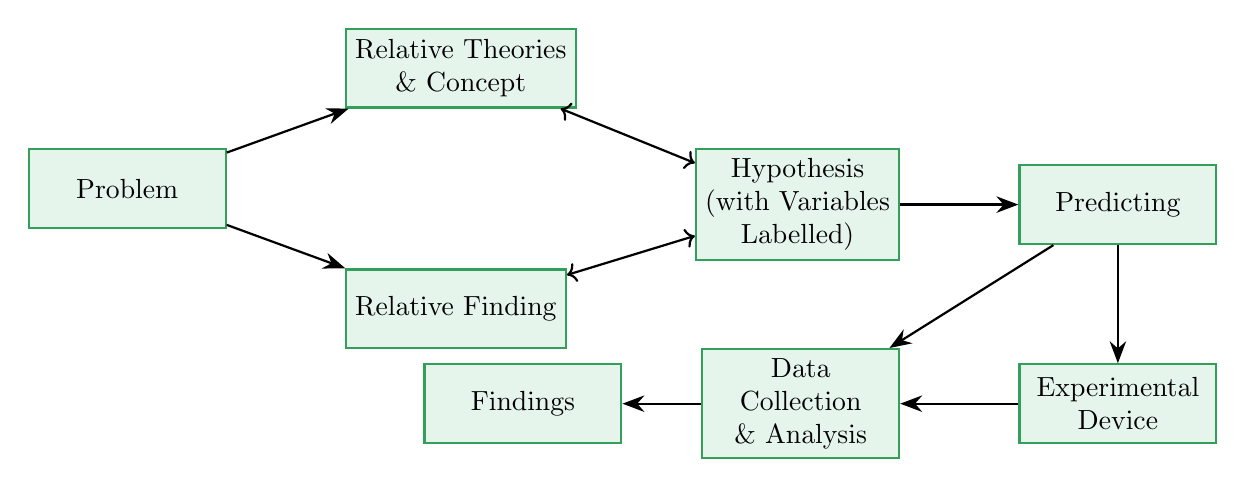
\begin{tikzpicture}[
        node distance=1.5cm and 1cm,
        box/.style={draw, rectangle, minimum width=2.5cm, minimum height=1cm, align=center, fill=tipbg, draw=tipframe, thick},
        arr/.style={-{Stealth[scale=1.2]}, thick}
    ]
    
    \node[box] (prob) {Problem};
    \node[box] (theory) [above right=0.5cm and 1.5cm of prob] {Relative Theories\\\& Concept};
    \node[box] (finding) [below right=0.5cm and 1.5cm of prob] {Relative Finding};
    \node[box] (hypo) [below right=0.5cm and 1.5cm of theory] {Hypothesis\\(with Variables\\Labelled)};
    \node[box] (pred) [right=1.5cm of hypo] {Predicting};
    \node[box] (exp) [below=1.5cm of pred] {Experimental\\Device};
    \node[box] (data) [left=1.5cm of exp] {Data\\Collection\\\& Analysis};
    \node[box] (res) [left=1cm of data] {Findings};

    \draw[arr] (prob) -- (theory);
    \draw[arr] (prob) -- (finding);
    \draw[<->, thick] (theory) -- (hypo);
    \draw[<->, thick] (finding) -- (hypo);
    \draw[arr] (hypo) -- (pred);
    \draw[arr] (pred) -- (exp);
    \draw[arr] (pred) -- (data);
    \draw[arr] (exp) -- (data);
    \draw[arr] (data) -- (res);

    \end{tikzpicture}
    \caption{Spektrum aliran penelitian dari masalah hingga penemuan.}
\end{figure}

\newpage
\section{Klasifikasi dan Macam-Macam Hipotesis}

Hipotesis menyatakan harapan peneliti mengenai hubungan antar variabel. Hipotesis ini bisa dipecah menjadi beberapa kelompok berdasarkan sifat matematis maupun arah hubungannya.

\subsection{Hipotesis Nol vs Hipotesis Alternatif}
Ketika kita melakukan eksperimen, kita membandingkan dua pernyataan statistik:
\begin{itemize}
    \item \textbf{Hipotesis Nol ($H_0$):} Sesuai namanya "nol", hipotesis ini menyatakan \textbf{tidak ada} perbedaan, tidak ada pengaruh, atau tidak ada hubungan antara variabel yang diteliti.
    \begin{itemize}
        \item \textit{Contoh:} "Tidak ada perbedaan waktu pencarian laman website antara pengguna menu \textit{pull-down} dan \textit{pop-up}".
    \end{itemize}
    \item \textbf{Hipotesis Alternatif ($H_a$ atau $H_1$):} Ini kebalikan dari $H_0$. Menyatakan bahwa \textbf{ada} perbedaan atau pengaruh yang nyata.
    \begin{itemize}
        \item \textit{Contoh:} "Ada perbedaan waktu pencarian laman website antara pengguna menu \textit{pull-down} dan \textit{pop-up}".
    \end{itemize}
\end{itemize}

\subsection{Hipotesis Direksional vs Non-Direksional}
Hipotesis juga bisa dibedakan berdasarkan apakah peneliti sudah yakin dengan "arah" hasil penelitiannya atau belum.

\begin{itemize}
    \item \textbf{Hipotesis Direksional (Berarah):} Peneliti dengan pede menetapkan arah perbedaannya (mana yang lebih tinggi, mana yang lebih rendah, mana yang lebih baik).
    \begin{itemize}
        \item \textit{Contoh:} "Siswa berkesulitan belajar yang menerima pembelajaran individu \textbf{akan memperoleh capaian belajar yang lebih tinggi} daripada siswa di pembelajaran kelompok".
    \end{itemize}
    \item \textbf{Hipotesis Non-Direksional (Tidak Berarah):} Peneliti cuma tahu pasti ada bedanya, tapi belum berani menetapkan arahnya ke mana.
    \begin{itemize}
        \item \textit{Contoh:} "Ada perbedaan capaian belajar antara siswa yang menerima pembelajaran individu dan pembelajaran kelompok".
    \end{itemize}
\end{itemize}

\newpage
\section{Perancangan Desain Eksperimen}

Desain eksperimen adalah level penelitian tertinggi kalau kita mau nyari \textit{sebab-akibat}. Dalam merancangnya, kita butuh pemahaman mendalam tentang komponen apa saja yang terlibat dan bagaimana cara membaginya.

\subsection{Tiga Komponen Utama Eksperimen}
Desain eksperimen dibangun dari tiga pondasi utama:
\begin{enumerate}
    \item \textbf{Perlakuan (Treatment / Kondisi):} Ini mengacu pada teknik, piranti, atau prosedur baru yang ingin diuji dan dibandingkan.
    \item \textbf{Unit Eksperimen:} Ini adalah objek yang bakal kita kasih perlakuan. Kalau di penelitian ranah IT seperti \textit{Human-Computer Interaction} (HCI), unitnya biasanya adalah subyek manusia (partisipan/user).
    \item \textbf{Metode Penugasan (Assignment Method):} Cara bagaimana kita menempatkan si unit (partisipan) tadi ke dalam kondisi perlakuan yang berbeda-beda.
\end{enumerate}

\subsection{Klasifikasi Kelompok Desain Penelitian}
Ada tiga kelompok desain penelitian eksperimental berdasarkan cara penugasan partisipannya:

\begin{figure}[h]
    \centering
    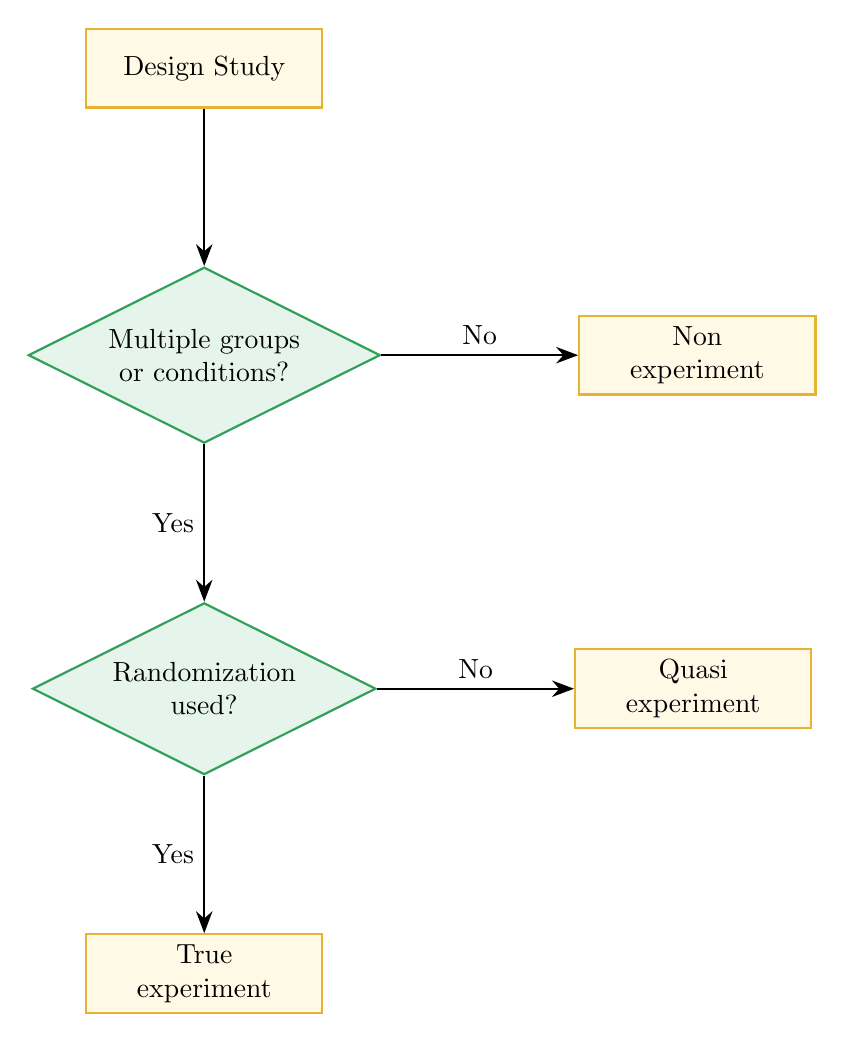
\begin{tikzpicture}[
        node distance=2cm and 2.5cm,
        box/.style={draw, rectangle, minimum width=3cm, minimum height=1cm, align=center, fill=notebg, draw=noteframe, thick},
        diam/.style={draw, diamond, aspect=2, align=center, fill=tipbg, draw=tipframe, thick},
        arr/.style={-{Stealth[scale=1.2]}, thick}
    ]
    
    \node[box] (start) {Design Study};
    \node[diam] (mult) [below=of start] {Multiple groups\\or conditions?};
    \node[box] (nonexp) [right=of mult] {Non\\experiment};
    
    \node[diam] (rand) [below=of mult] {Randomization\\used?};
    \node[box] (quasi) [right=of rand] {Quasi\\experiment};
    
    \node[box] (true) [below=of rand] {True\\experiment};

    \draw[arr] (start) -- (mult);
    \draw[arr] (mult) -- node[above] {No} (nonexp);
    \draw[arr] (mult) -- node[left] {Yes} (rand);
    \draw[arr] (rand) -- node[above] {No} (quasi);
    \draw[arr] (rand) -- node[left] {Yes} (true);

    \end{tikzpicture}
    \caption{Alur logika penentuan desain penelitian.}
\end{figure}

\newpage
\section{Strategi Penugasan Partisipan}

Dalam mendesain eksperimen, misal kita mau membandingkan kecepatan ngetik pakai tiga tipe keyboard (QWERTY, DVORAK, Alphabet), kita harus milih strategi pembagian kelompok. Ada dua gaya utama:

\subsection{Desain Antar-Kelompok (Between-Group)}
Di desain ini, setiap partisipan \textbf{hanya dikenai satu kondisi} eksperimen aja. Jadi kalau ada 3 tipe keyboard, orangnya kita bagi jadi 3 kelompok terpisah. Masing-masing kelompok murni cuma nyobain 1 keyboard aja.
\begin{itemize}
    \item \textbf{Keuntungan:} Menghindari \textit{learning effect} (pengaruh belajar). Orang nggak bakal hapal pola teksnya karena mereka cuma ngetik pakai satu jenis keyboard.
    \item \textbf{Kerugian:} Butuh ukuran sampel (jumlah orang) yang sangat besar biar hasilnya imbang.
\end{itemize}

\subsection{Desain Dalam-Kelompok (Within-Group)}
Di desain ini, setiap partisipan akan \textbf{dikenai semua kondisi} eksperimen. Artinya, satu grup yang sama akan disuruh nyoba ngetik pakai QWERTY, lalu lanjut pakai DVORAK, lalu lanjut lagi pakai Alphabet.
\begin{itemize}
    \item \textbf{Keuntungan:} Nggak butuh orang banyak (ukuran sampel bisa kecil), karena orang yang sama dipakai berulang kali.
    \item \textbf{Kerugian:} Rentan terkena \textit{learning effect}. Pas dia nyoba keyboard ketiga, bisa jadi dia ngetiknya lebih cepet bukan karena keyboardnya bagus, tapi karena dia udah hapal sama teks yang diketik dari percobaan pertama.
\end{itemize}

\newpage
\section{Desain Faktorial dan Pengaruh Interaksi}

\subsection{Menyelidiki Lebih dari Satu Variabel Independen}
Kadang, masalah di dunia nyata itu nggak sesederhana satu lawan satu. Gimana kalau kita mau menguji pengaruh Keyboard Type (QWERTY, DVORAK, Alphabet) \textbf{DAN} juga Task Type (Tugas Menyalin vs Tugas Mengarang) secara bersamaan terhadap kecepatan ngetik?

Kondisi ini disebut dengan \textbf{Desain Faktorial}. Peneliti mengawinkan berbagai level dari tiap variabel independen.
Karena ada 3 tipe keyboard dan 2 tipe tugas, totalnya ada $3 \times 2 = 6$ kondisi uji coba yang harus dilewati:

\begin{table}[h]
\centering
\begin{tabular}{@{}lccc@{}}
\toprule
\textbf{Tipe Tugas} & \textbf{QWERTY} & \textbf{DVORAK} & \textbf{Alphabet} \\ \midrule
\textbf{Mengarang} & Kondisi 1 & Kondisi 2 & Kondisi 3 \\
\textbf{Menyalin} & Kondisi 4 & Kondisi 5 & Kondisi 6 \\ \bottomrule
\end{tabular}
\caption{Matriks Desain Faktorial 3x2}
\end{table}

\subsection{Membedah Pengaruh Interaksi (Interaction Effect)}
Keuntungan pakai Desain Faktorial adalah kita bisa melihat \textbf{Pengaruh Interaksi}. Pengaruh interaksi terjadi kalau ternyata \textit{efek dari suatu variabel independen itu bergantung pada kondisi variabel independen lainnya}.

\begin{notebox}
\textbf{Contoh Kasus Efek Interaksi:}\\
Seorang dosen membandingkan efektivitas "Metode Diskusi" vs "Metode Ceramah". Setelah diuji bareng, hasilnya sama rata. \textbf{Tapi}, dosen tersebut menduga bahwa "Metode Diskusi" itu jauh lebih cocok buat Mahasiswa Wanita, sedangkan "Metode Ceramah" lebih cocok buat Mahasiswa Pria.
\end{notebox}

Jika kita plot data tersebut ke dalam grafik prestasi, kita akan melihat garis yang bersilangan tajam. Garis yang saling silang ini adalah bukti telak adanya Pengaruh Interaksi. Kalau data Pria dan Wanita cuma digabung (nggak dipecah), perbedaannya bakal saling menghilangkan dan seolah-olah kedua metode itu ngasih efek yang sama.

\begin{figure}[h]
    \centering
    \begin{tikzpicture}[scale=1.2]
        % Axes
        \draw[->, thick] (0,0) -- (8,0) node[right] {Metode Pembelajaran};
        \draw[->, thick] (0,0) -- (0,5) node[above] {Prestasi};
        
        % Labels
        \node[below] at (2,0) {Diskusi};
        \node[below] at (6,0) {Ceramah};
        
        % Lines
        \draw[blue, thick] (1,4.5) -- (7,1.5) node[right, text=black] {Wanita};
        \draw[red, thick] (1,1.5) -- (7,4.5) node[right, text=black] {Pria};
        
        % Text on lines
        \node[above] at (2.5, 3.8) {Wanita};
        \node[below] at (2.5, 2.2) {Pria};

    \end{tikzpicture}
    \caption{Grafik Pengaruh Interaksi. Garis bersilang menunjukkan interaksi kuat antara Metode Pembelajaran dan Gender terhadap Prestasi.}
\end{figure}

\end{document}